%这是LaTeX源文件
%编译要求:
%编译命令: xelatex -shell-escape rep.tex
%其他要求: 需要安装字体Bitstream Vera Sans Mono;需要安装pygments;需要文档类'cumtbrep';需要实验中用到的代码文件

\documentclass{cumtbrep}

\usepackage{float}
\usepackage{graphicx}
\usepackage{amsmath}
%hyper ref
\usepackage{hyperref}
\hypersetup{colorlinks,bookmarks=false,pdfauthor=王凌峰,pdftitle=报告1~3}
%font spec
\usepackage{fontspec}
\newfontfamily\bvsm{Bitstream Vera Sans Mono}[NFSSFamily=bvsmfamily]
%code
\usepackage{listings}
\usepackage{minted}
\setminted{breaklines,breakanywhere,mathescape,tabsize=4,style=default,fontsize=\normalsize,fontfamily=bvsmfamily,linenos}
%codes' line number format
\renewcommand{\theFancyVerbLine}{\sffamily
\textcolor[rgb]{0.5,0.5,0.5}{\scriptsize\oldstylenums{\arabic{FancyVerbLine}}}}
%listing's caption
\usepackage{caption}
\captionsetup{tablename=code}
%code with caption
\newcommand\inputcode[3][c++]{%
	\inputminted{#1}{#2}
	\begin{figure}[H]
		\centering
		\captionsetup{type=table}
		\caption{\texttt{#3}}
	\end{figure}
}
\newcommand\inline[1]{\mintinline{c++}{#1}}

\begin{document}

\makeheader{计算机图形学}{王振武}{计科\numberstyle 19-2}{王凌峰}{\numberstyle 1910630221}

\namesec
\begin{enumerate}
	\item \hyperref[sec:1]{画直线}
	\item \hyperref[sec:2]{画圆}
	\item \hyperref[sec:3]{多边形填充}
\end{enumerate}

\purposesec
\noindent 选一种方法

\contentsec
\section*{说明}
这些PDF文件没有对应的Word版本,因为是用 \LaTeX{} 写的。源文件在 \path{tex}文件夹。

实验中使用OpenGL core mode,版本要求3.3及以上。Context creation使用GLFW,function loading使用glbinding。不使用Visual Studio。

\section{画直线}\label{sec:1}
用中点法。

实际上OpenGL的rasterization是不可编程的,只能先在CPU生成一系列坐标,作为vertices输入GPU,以point primitive绘制来模拟rasterization。实验1和实验2都是这么干的。本实验中rasterization的模拟放在 \path{line.cc}中。

目录结构:{\ttfamily \lstinputlisting{../line/tree}}

之后的实验中只有新增或修改文件时才贴出代码,目录结构中没有给出代码的文件默认与下面贴出的代码相同。文件名标在完整代码的下方。

由于使用OpenGL core mode,shader需要自己编写。\path{trivial.vert}和 \path{trivial.frag}分别为vertex shader和fragment shader。\texttt{shader}类的作用是读取、编译shader,与program连接,并对错误做必要处理。
\inputcode{../line/shader.hh}{shader.hh}

\texttt{shader}类从文件读取vertex shader和fragment shader:
\inputcode{../line/shader.cc}{shader.cc}

我设定窗口大小为$1920\times 1028$,以屏幕左下角为原点。为了将$[0,1919]\times [0,1027]$内的点变换到$[-1,1]^3$,先把输入点用homogeneous coordinate表示,再通过orthographic projection transformation将其变换到NDC。这是一个简单的windowing transform:
\[
	\mathbf{M}_{\mathit{orth}} = \begin{bmatrix}
		\frac{2}{r-l} & 0 & 0 & \frac{l+r}{r-l} \\
		0 & \frac{2}{t-b} & 0 & \frac{b+t}{b-t} \\
		0 & 0 & \frac{2}{n-f} & \frac{f+n}{f-n} \\
		0 & 0 & 0 & 1
	\end{bmatrix}
\]

$l, r, b, t, n, f$分别为左、右、底、顶、近、远处在各个方向的坐标。这个实验不涉及$z$轴,$n$和$f$的取值是无所谓的。为了方便分别取$0$和$-1$。

$\mathbf{M}_{\mathit{orth}}$不会变化,所以直接编码在vertex shader内:
\inputcode[glsl]{../line/trivial.vert}{trivial.vert}

fragment shader直接返回黑色:
\inputcode[glsl]{../line/trivial.frag}{trivial.frag}

顶点数据,即模拟rasterization得到的点向GPU的输入使用现代的VAO和VBO,每个VAO关联一组vertices,代表一条测试直线的rasterization的结果。测试覆盖了直线斜率的各种情况,共6条。

\path{main.cc}中先进行窗口初始化和函数绑定,然后编译、连接得到program。调用 \inline{line_rasterizer}得到测试线rasterization结果,在GPU中创建buffer并存入。在主循环中清除color buffer,依次绑定每个VAO并绘制与VAO绑定的VBO中的点:
\inputcode{../line/main.cc}{main.cc}

下面是 \path{line.hh}:\inputcode{../line/line.hh}{line.hh}

\inline{line_rasterizer}接受一个函数指针,可以传入mid-point或bresenham方法。

当$0<k\le 1$不满足时,或可以直接给出结果($k=0$或$k\to\infty$),或可以转换为$0<k\le 1$的情形。

$k=0$或$k\to\infty$的情形是非常简单的。\inline{line_rasterizer}中的代码直接处理这个平凡的情形。

当$|k|>1$时,需要互换$x,y$。为了结果正确,以 \inline{reversed}标记存入结果时是否需要互换坐标位置。

为了处理方便,称其中一条坐标轴为参考轴,规定处理过程中点在参考轴上的坐标只能增加。另一条坐标轴称为非参考轴,点在非参考轴的坐标变化没有限制。输入确定直线的两点后,以参考轴坐标较小的点为起点,每次将参考轴坐标增$1$,计算应有的非参考轴坐标,直到参考轴坐标超过参考轴坐标较大的点的参考轴坐标。

所以需要知道非参考轴坐标如何计算。容易看出,
\begin{itemize}
	\item 若$k<0$,非参考轴坐标随参考轴坐标增加而\textbf{减小或不变}
	\item 若$k>0$,非参考轴坐标随参考轴坐标增加而\textbf{增加或不变}
\end{itemize}

因此可根据$k$判断非参考轴的增减性,这个性质用 \inline{asc}标记。增减性不同时$d$的初始值和增量也不同,对于$Ax+By+C=0$形式的直线,
\begin{itemize}
	\item 若 \inline{asc==true}: $\Delta d = A+B(d<0) \quad \text{or} \quad \Delta d=A(d\ge 0)$
	\item 若 \inline{asc==false}: $\Delta d = A(d<0) \quad \text{or} \quad \Delta d=A-B(d\ge 0)$
\end{itemize}

\inline{line_rasterizer}中判断$k$的值,给 \inline{asc}和 \inline{reversed}赋合适的值,传入mid-point或bresenham方法的函数。

具体处理$0<k<1$情形的函数则根据这些参数决定$\Delta d$以及存入点坐标的次序。

\inputcode{../line/line.cc}{line.cc}

\section{画圆}\label{sec:2}
用中点法。

与上个实验相同,绘制点模拟rasterization。

目录结构:{\ttfamily \lstinputlisting{../circle/tree}}
rasterization代码在 \path{circle.cc}中。

\path{main.cc}和实验一类似,测试了6个圆。
\inputcode{../circle/main.cc}{main.cc}
\inputcode{../circle/circle.hh}{circle.hh}

课本中从$(0,R)$开始顺时针计算$1/8$个圆,再对这部分点对称变换得到剩余部分。但$y$轴上和直线$y=x$上的点沿自身所在直线对称变换后得到自身,导致冗余。所以这里对点$(0,R)$单独对称变换,而$1/8$圆的计算从$(1,R)$或$(1,R-1)$开始,到$x\ge y$为止。$1/8$圆计算结束时若$x=y$,还要将直线$y=x$上的点沿$x$轴和$y$轴对称。

因此一个圆需要的点的数量为$(\lfloor R/\sqrt{2}\rfloor*8+4)$或$(\lfloor R/\sqrt{2}\rfloor*8+8)$。

对于圆心$\vec o$不在$(0,0)$的圆,计算出的任意一点位置向量加上$\vec o$即可。
\inputcode{../circle/circle.cc}{circle.cc}

\section{多边形填充}\label{sec:3}
用4-邻接的种子填充法。

目录结构:{\ttfamily \lstinputlisting{../filling/tree}}
为了方便,用 \texttt{point}类表示点。
\inputcode{../filling/point.hh}{point.hh}
\inputcode{../filling/point.cc}{point.cc}

\path{main.cc}中测试了4边形的填充:
\inputcode{../filling/main.cc}{main.cc}

\inputcode{../filling/fill.hh}{fill.hh}

\inline{fill_poly}中点存在 \inline{std::set}中。首先把多边形每个点根据顺序两两配对,调用 \inline{add_edge_points}把这两点所表示的直线rasterize。

填充起始点$(x_0,y_0)=\frac{1}{n}\sum\limits_{i=1}^{n}(x_i,y_i)$,$n$为多边形顶点个数。这保证了起始点在多边形内部,但只保证对凸多边形有效。

在 \inline{std::set}中的点表示已填充的点。填充过程中出栈一个点,把每个不在 \inline{std::set}中且不在栈中的这个点的4-邻接点入栈,直到栈空就完成了填充。
\inputcode{../filling/fill.cc}{fill.cc}

\analysesec
\begin{figure}[H]
	\centering
	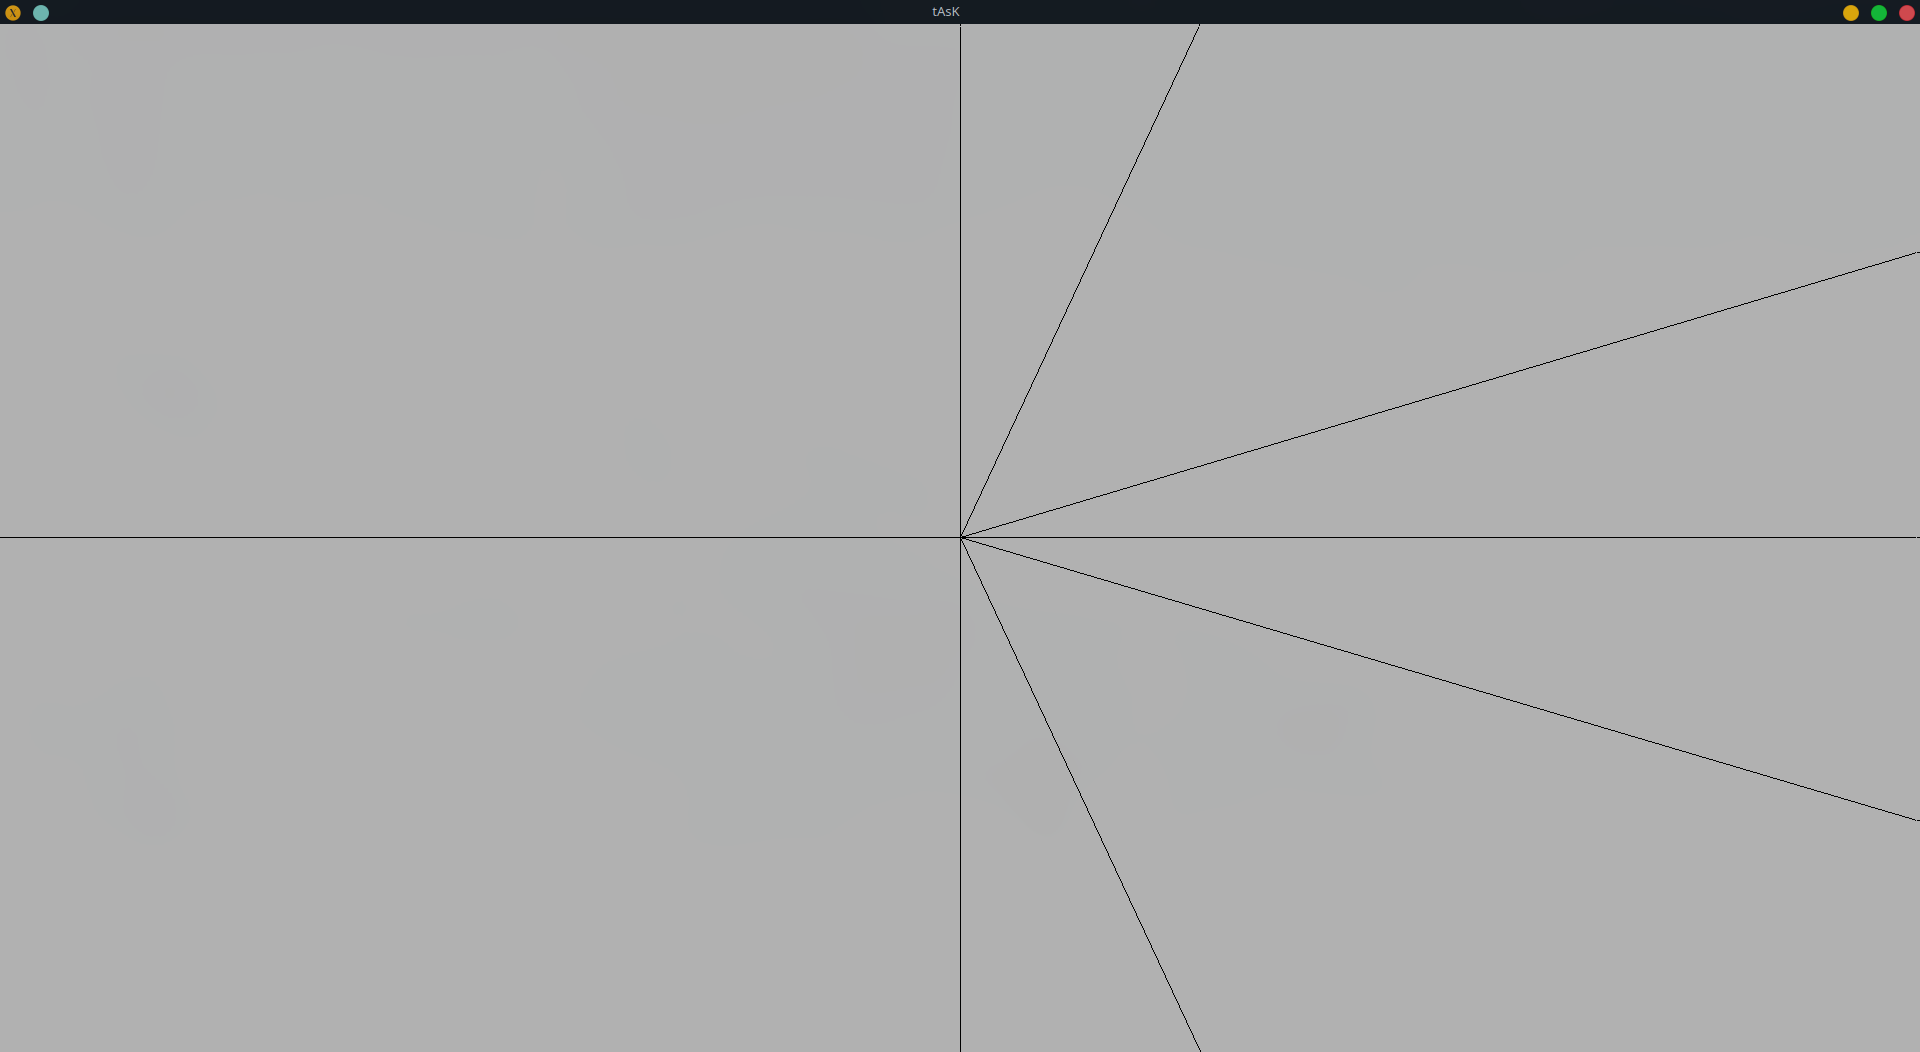
\includegraphics[scale=0.25]{../line/line.png}
	\caption{画直线}
\end{figure}
\begin{figure}[H]
	\centering
	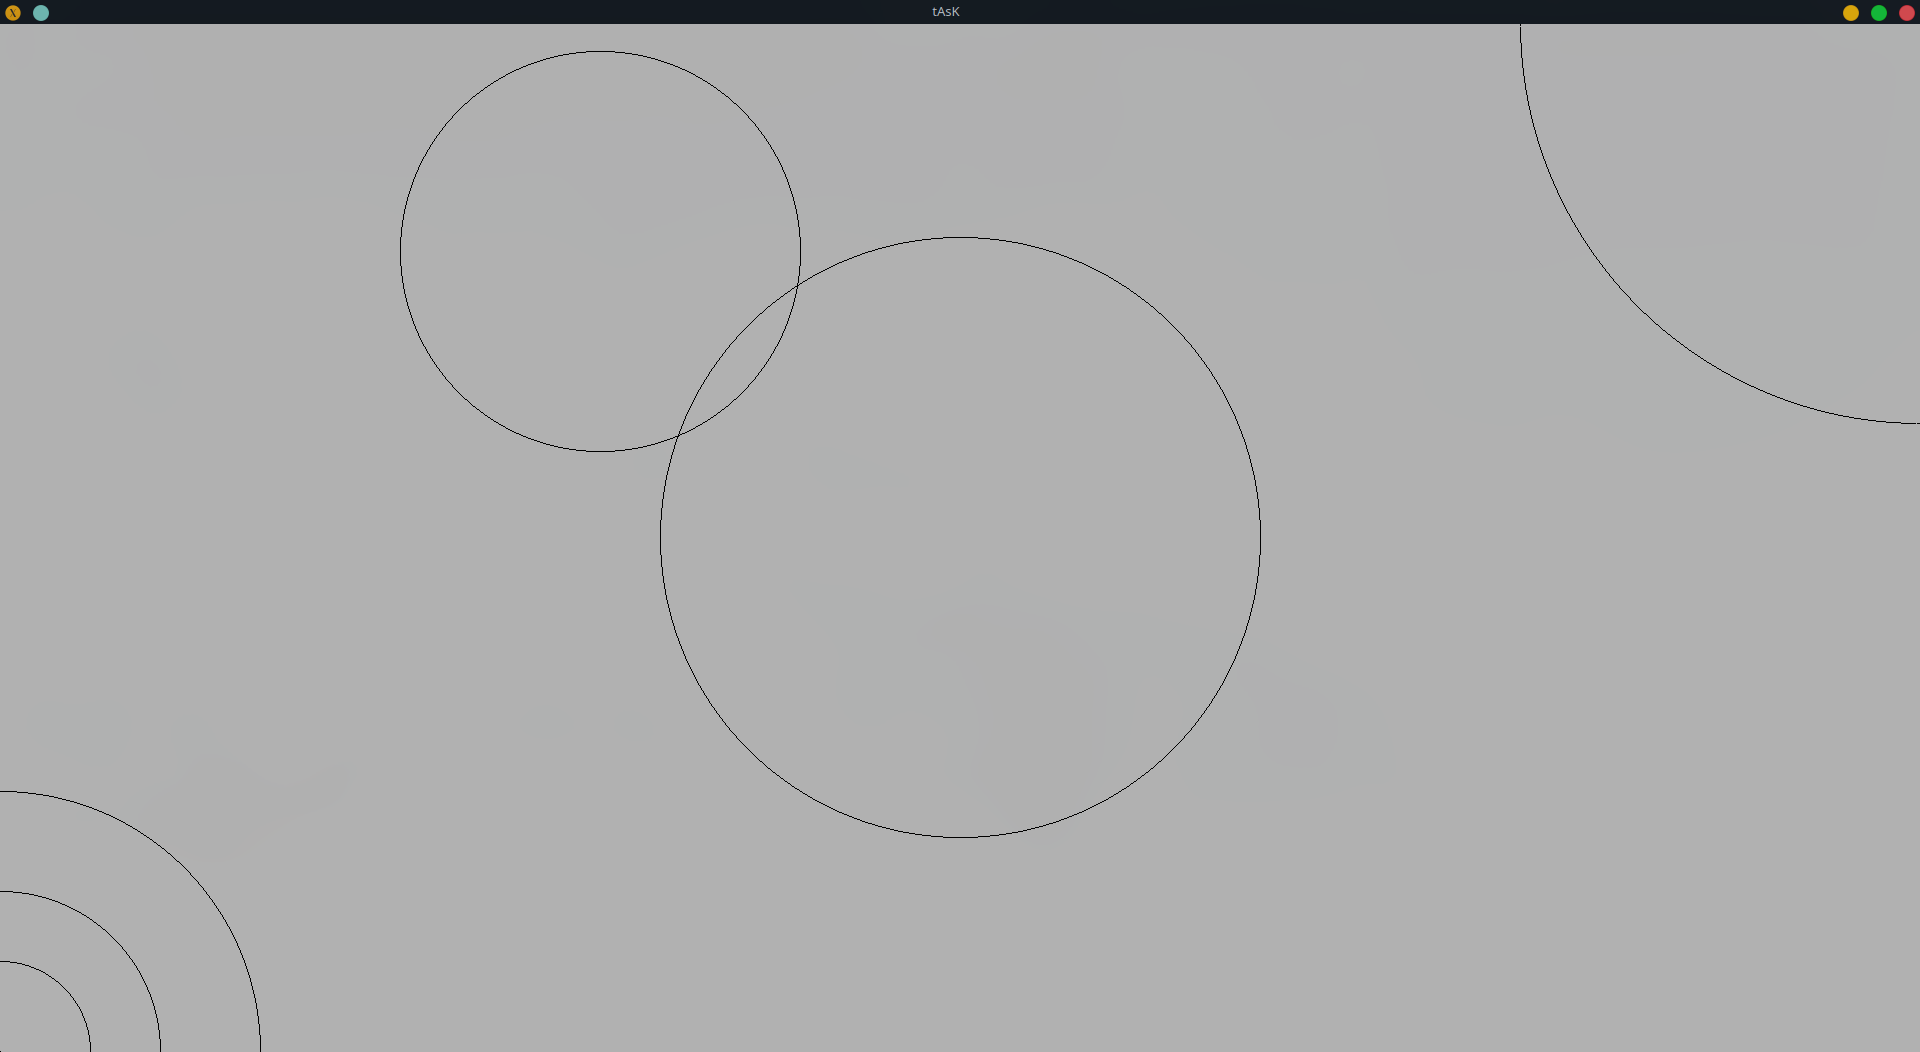
\includegraphics[scale=0.25]{../circle/circle.png}
	\caption{画圆}
\end{figure}
\begin{figure}[H]
	\centering
	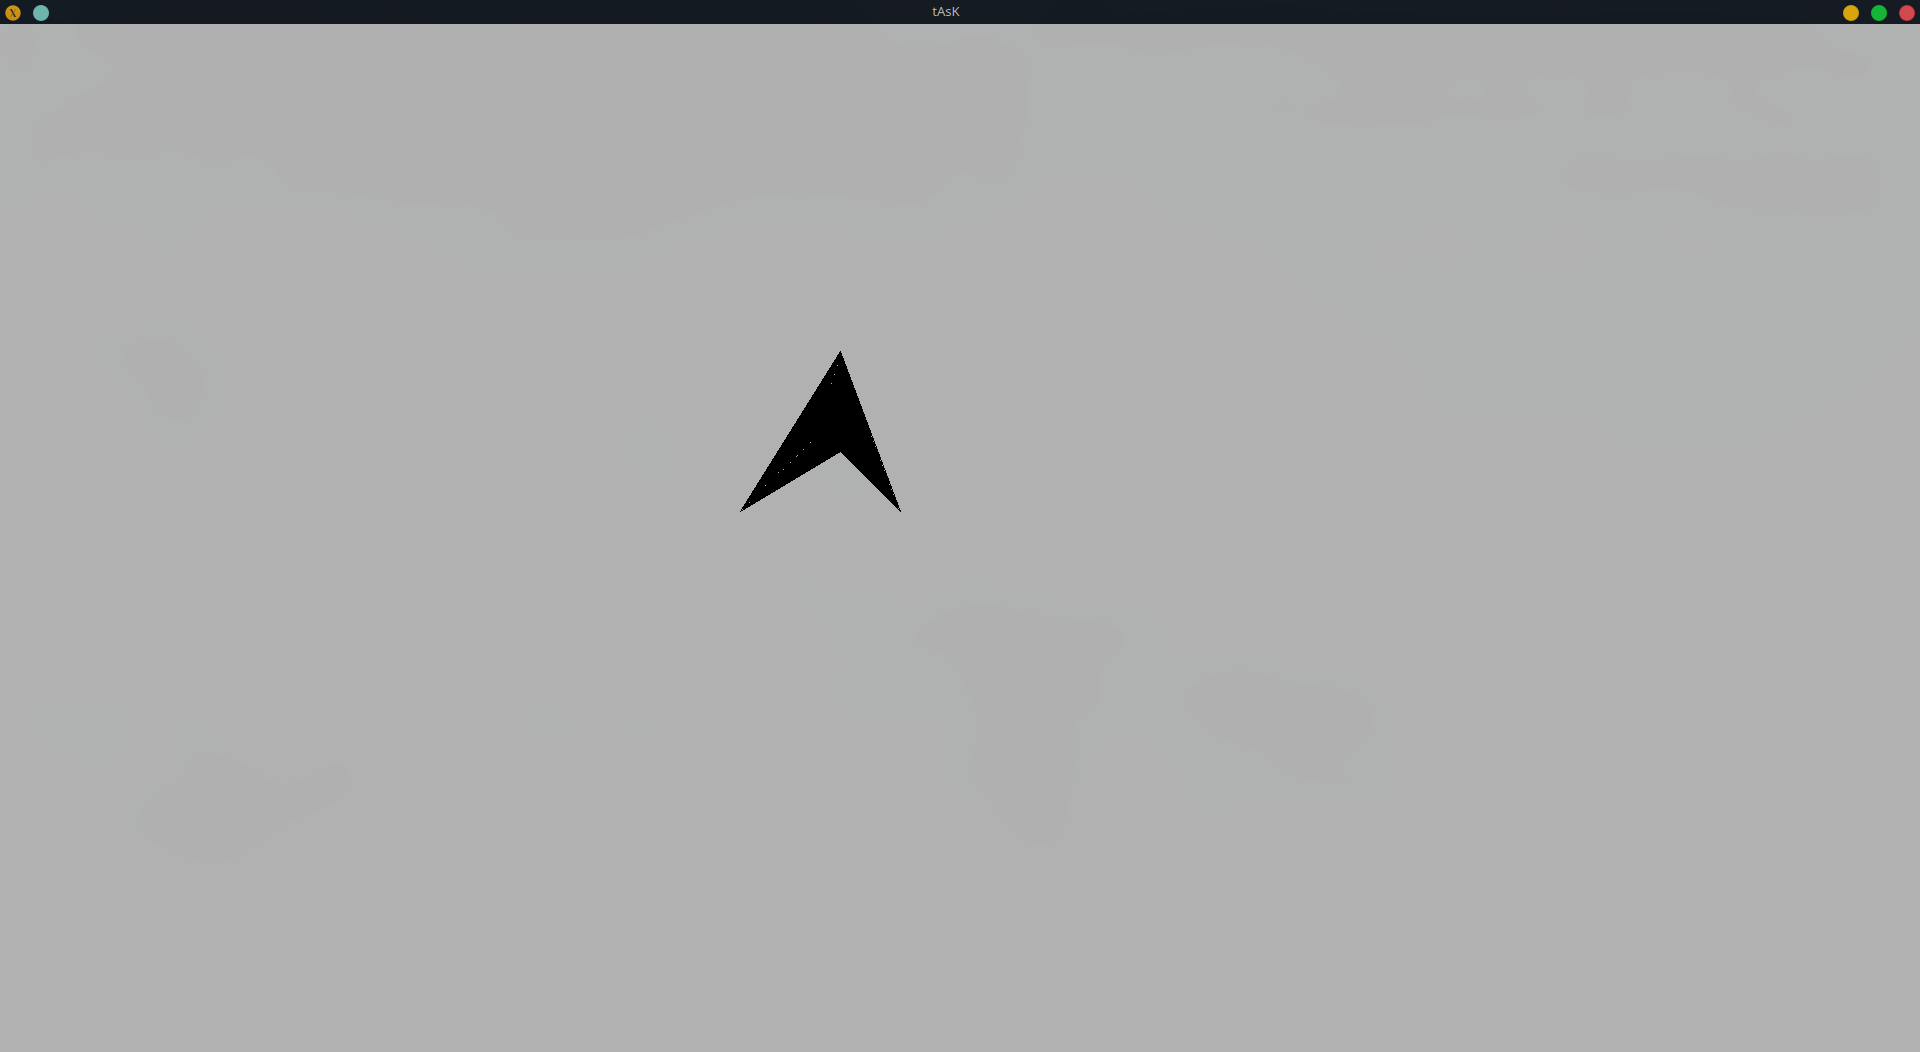
\includegraphics[scale=0.25]{../filling/filling.png}
	\caption{填充}
\end{figure}

\maketail

\end{document}
